\chapter{Меры близости (ЛР2)}

\section{Методика выбора мер}
\label{sec:lr2_method}

Все меры в работе приводятся к одной шкале близости. Значение $\mathrm{sim}(x,y)$ лежит в $[0,1]$, причём $\mathrm{sim}(x,x)=1$ и $\mathrm{sim}(x,y)=\mathrm{sim}(y,x)$. Если мерой является расстояние, оно нормируется в $[0,1]$ и переводится в близость как $\mathrm{sim} = 1 - d$~\cite{bolshakova2011}. Числовые признаки предварительно нормируются по каталогу методом min-max по формуле $x' = (x - \min)/(\max - \min)$. Без нормировки сахар с размахом 320 г/л подавил бы объём бутылки с размахом 0,5 л.

Признаки разнотипны, и единой меры для всего вектора нет. Для каждого типа выбирается своя частная мера, а затем строится обобщающая мера как их взвешенная сумма. Выбор между кандидатами одного типа проводится в три шага.
\begin{enumerate}[leftmargin=1.6\parindent]
	\item Для каждой меры строится матрица смежности $G_{ij} = g(o_i, o_j)$ размера $30\times30$ по всем парам объектов.
	\item По матрице строится тепловая карта. На ней видно, выделяет ли мера блоки родственных объектов и насколько зернистая её шкала.
	\item Карты и численные показатели сравниваются между собой. Это значения на эталонных парах заведомо похожих и заведомо различных ликёров, согласованность ранжирований пар по коэффициенту Спирмена $\rho$ для 435 пар верхнего треугольника~\cite{spearman1904} и число уникальных значений. Чем уникальных значений меньше, тем больше пар неразличимы.
\end{enumerate}

Расчёт выполняет скрипт \code{2-metrics/metrics.py}. Матрицы сохраняются в CSV, Excel и интерактивную HTML-страницу \code{out/matrices.html}, а тепловые карты --- в PNG.

\section{Числовые признаки}

Кандидаты --- семейство Минковского $d_p = \bigl(\tfrac{1}{D}\sum_{k}|x_k-y_k|^p\bigr)^{1/p}$ при $p = 1, 2, 3$ и $\infty$, то есть манхэттенская, евклидова, мера Минковского и мера Чебышёва. Пятым кандидатом выступает косинусное расстояние $d = 1 - \frac{x\cdot y}{\|x\|\,\|y\|}$. Множитель $1/D$ при трёх осях нормирует все меры в $[0,1]$. Значения на эталонных парах приведены в таблице~\ref{tab:lr2_numeric}, а согласованность и зернистость --- в таблице~\ref{tab:lr2_numeric_stats}.

\begin{table}[H]
	\centering
	\caption{Числовые меры расстояния на эталонных парах}
	\label{tab:lr2_numeric}
	\footnotesize\setlength{\tabcolsep}{4pt}
	\begin{tabular}{|L{1.6cm}|c|c|c|c|c|L{4.0cm}|}
		\hline
		Пара & $p=2$ & $p=1$ & $p=3$ & $p=\infty$ & cos & Смысл пары \\ \hline
		L26--L27 & 0,000 & 0,000 & 0,000 & 0,000 & 0,000 & какао-ликёры, числа совпадают \\ \hline
		L08--L10 & 0,025 & 0,015 & 0,030 & 0,044 & 0,001 & Cointreau / Grand Marnier \\ \hline
		L20--L21 & 0,036 & 0,021 & 0,043 & 0,063 & 0,001 & два амаретто \\ \hline
		L15--L16 & 0,101 & 0,058 & 0,121 & 0,175 & 0,025 & абрикос / персик \\ \hline
		L06--L30 & 0,452 & 0,369 & 0,484 & 0,563 & 0,614 & Fernet / Advocaat \\ \hline
		L04--L13 & 0,581 & 0,377 & 0,694 & 1,000 & 0,452 & крайние по крепости, 55 и 15 \% \\ \hline
	\end{tabular}
\end{table}

\begin{table}[H]
	\centering
	\caption{Согласованность ранжирований пар по Спирмену $\rho$ и зернистость шкалы}
	\label{tab:lr2_numeric_stats}
	\footnotesize
	\begin{tabular}{|l|c|c|c|L{2.3cm}|L{1.8cm}|}
		\hline
		Мера & $\rho$ с $p=2$ & $\rho$ с $p=\infty$ & $\rho$ с cos & Уникальных из 435 & Пар в связках \\ \hline
		евклидова ($p=2$) & --- & 0,970 & 0,881 & 354 & 148 \\ \hline
		манхэттенская ($p=1$) & 0,974 & 0,903 & 0,906 & 227 & 310 \\ \hline
		Минковского ($p=3$) & 0,995 & 0,987 & 0,857 & 359 & 141 \\ \hline
		Чебышёва ($p=\infty$) & 0,970 & --- & 0,809 & 92 & 406 \\ \hline
		косинусная & 0,881 & 0,809 & --- & 406 & 57 \\ \hline
	\end{tabular}
\end{table}

На эталонных парах порядок <<близко --- далеко>> у всех мер правильный, поэтому решают свойства шкалы.
\begin{itemize}[leftmargin=1.6\parindent, label*=---]
	\item \textbf{Чебышёв отвергнут.} Мера видит только координату с наибольшей разностью. В результате 93\,\% пар попадают в связки, всего 92 уникальных значения на 435 пар. У Baileys и Amarula совпадают крепость и почти совпадает сахар. Однако расстояние 0,5 целиком определяется объёмом бутылки, 1,0 л против 0,75 л. Для пары L04--L13 расстояние 1,0 задано только крепостью, а сахар не учитывается вовсе.
	\item \textbf{Минковский $p=3$ отвергнут} как промежуточный шаг к Чебышёву. Его ранжирование почти совпадает с чебышёвским, $\rho = 0{,}987$, а нового смысла по сравнению с $p=2$ он не даёт.
	\item \textbf{Косинусная мера отвергнута.} Она сравнивает направление вектора, а не величину. Пропорциональные, но разные векторы получают расстояние 0. Например, ликёр вдвое крепче и вдвое слаще оказался бы <<тем же самым>>. Это нарушает аксиому $d(x,y) = 0 \Leftrightarrow x = y$. На близких парах мера слишком оптимистична и даёт 0,001 для L08--L10, а с остальными мерами она согласуется хуже всех.
	\item \textbf{Евклидова мера выбрана} вместо манхэттенской. Ранжирования почти совпадают, $\rho = 0{,}974$. Однако у евклидовой меры вклад разности квадратичный. Одно крупное отличие вроде 20 п.\,п. крепости штрафуется сильнее, чем та же сумма, распределённая по осям. Для ликёров это верно, потому что большая разница в крепости важнее нескольких мелких отличий. Кроме того, евклидова мера --- единственная изотропная $L_p$-норма, а её шкала зернистее, 354 уникальных значения против 227.
\end{itemize}

\begin{figure}[H]
	\centering
	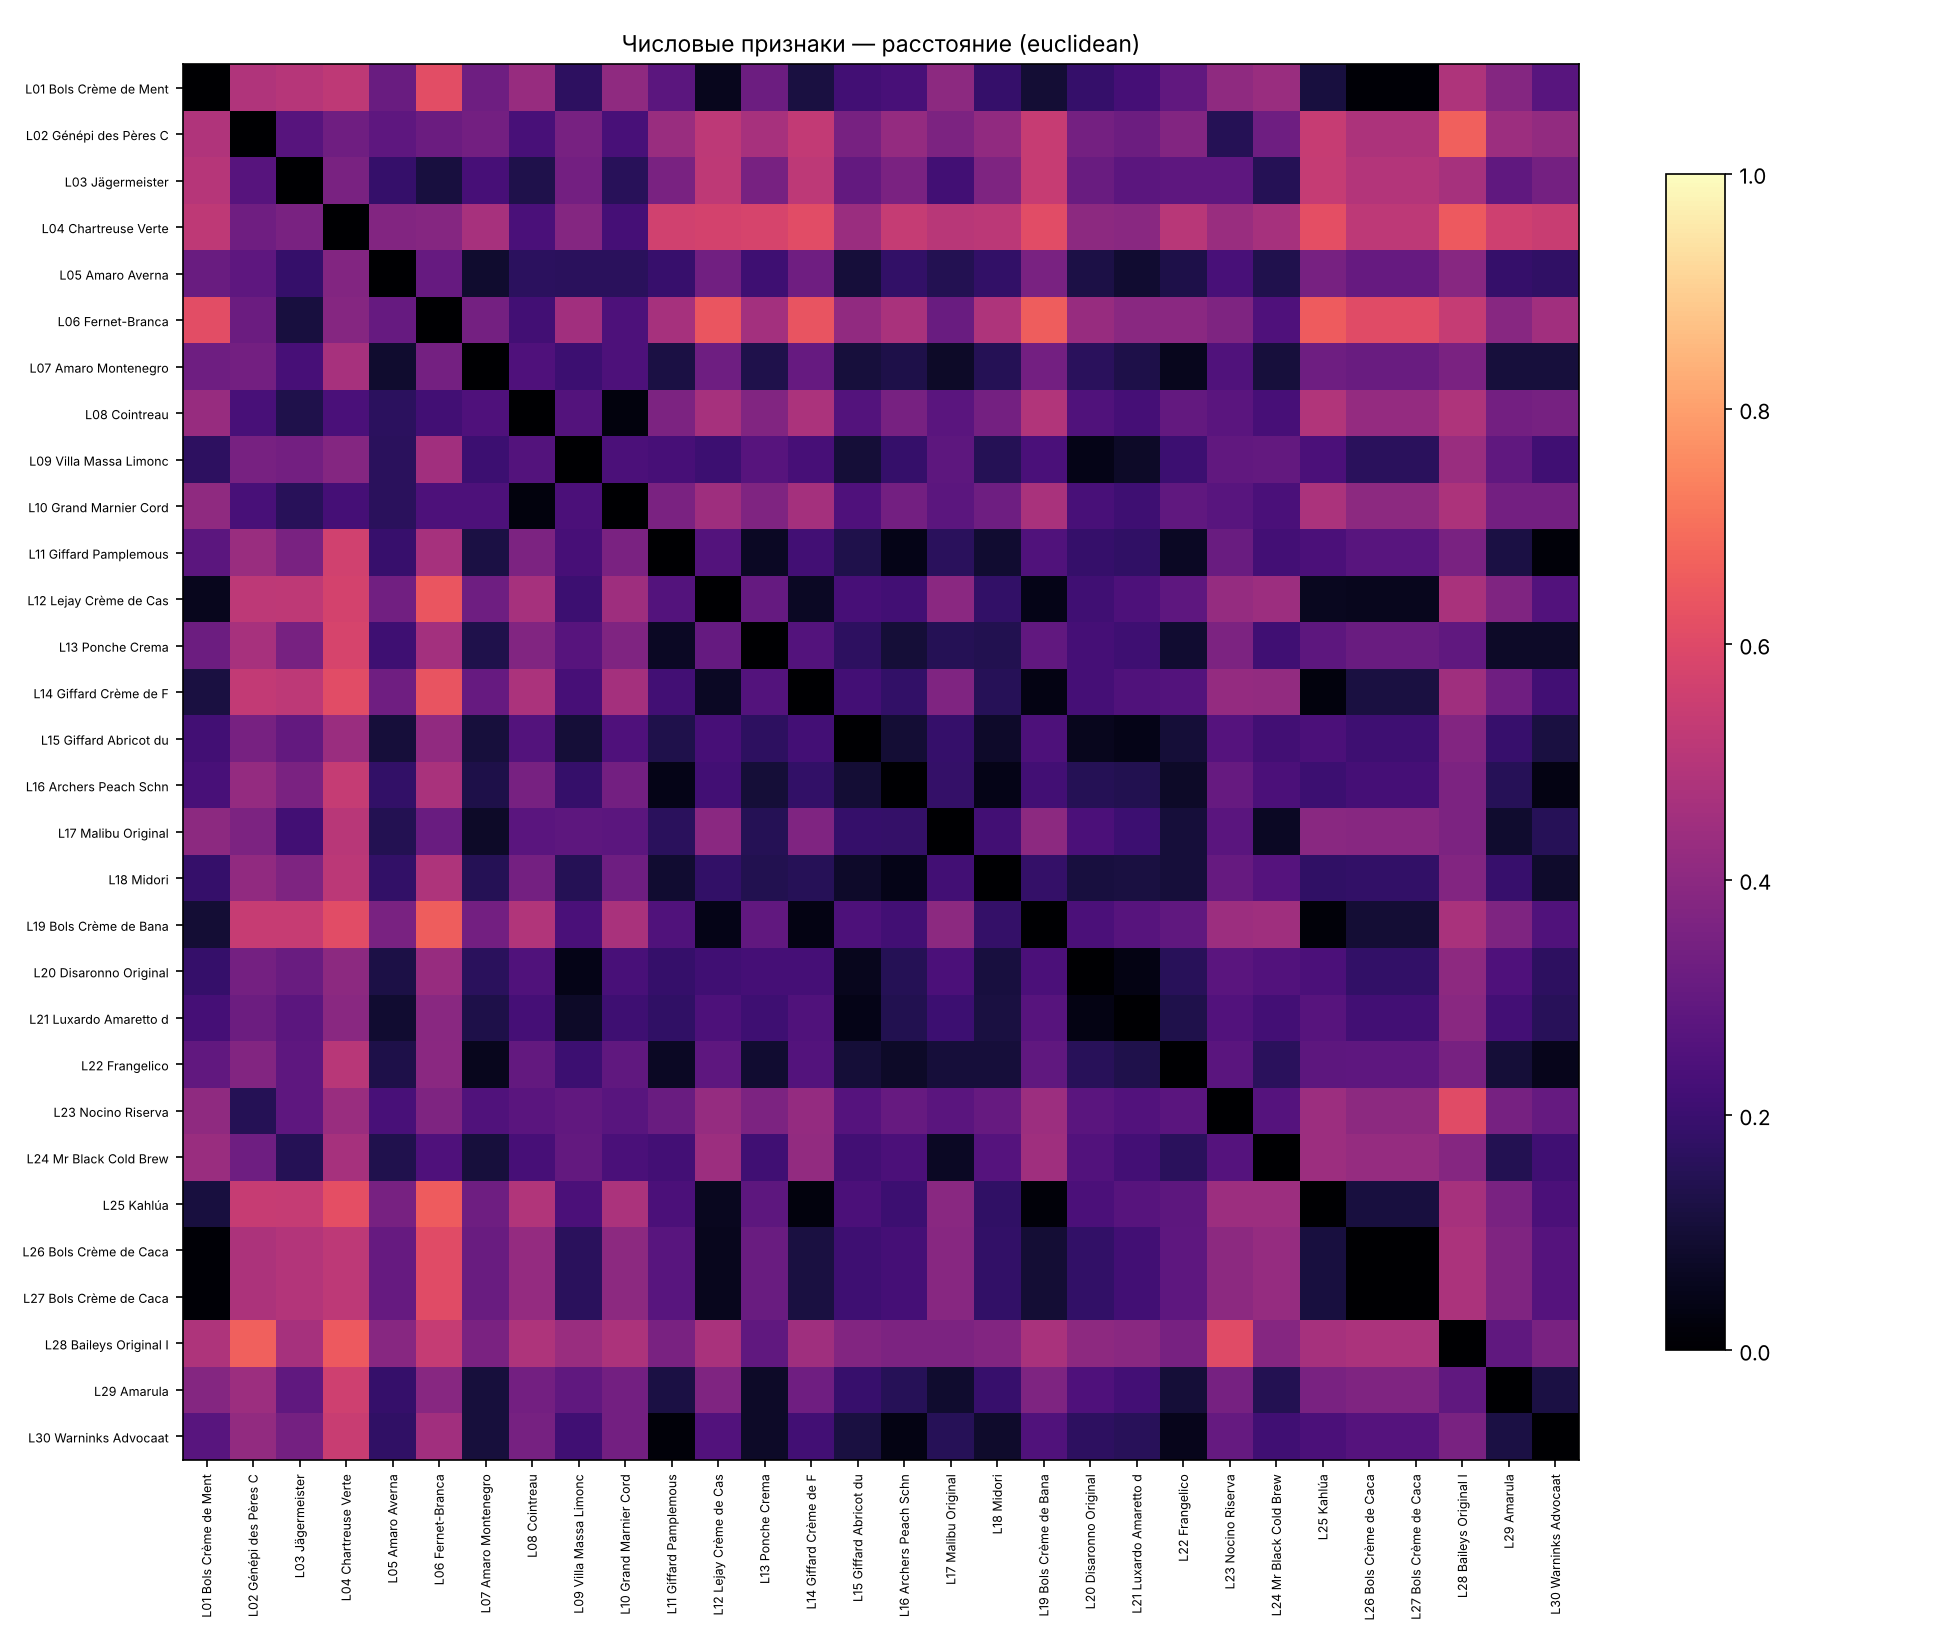
\includegraphics[width=0.32\textwidth]{lr2/num_euclidean_dist.png}\hfill
	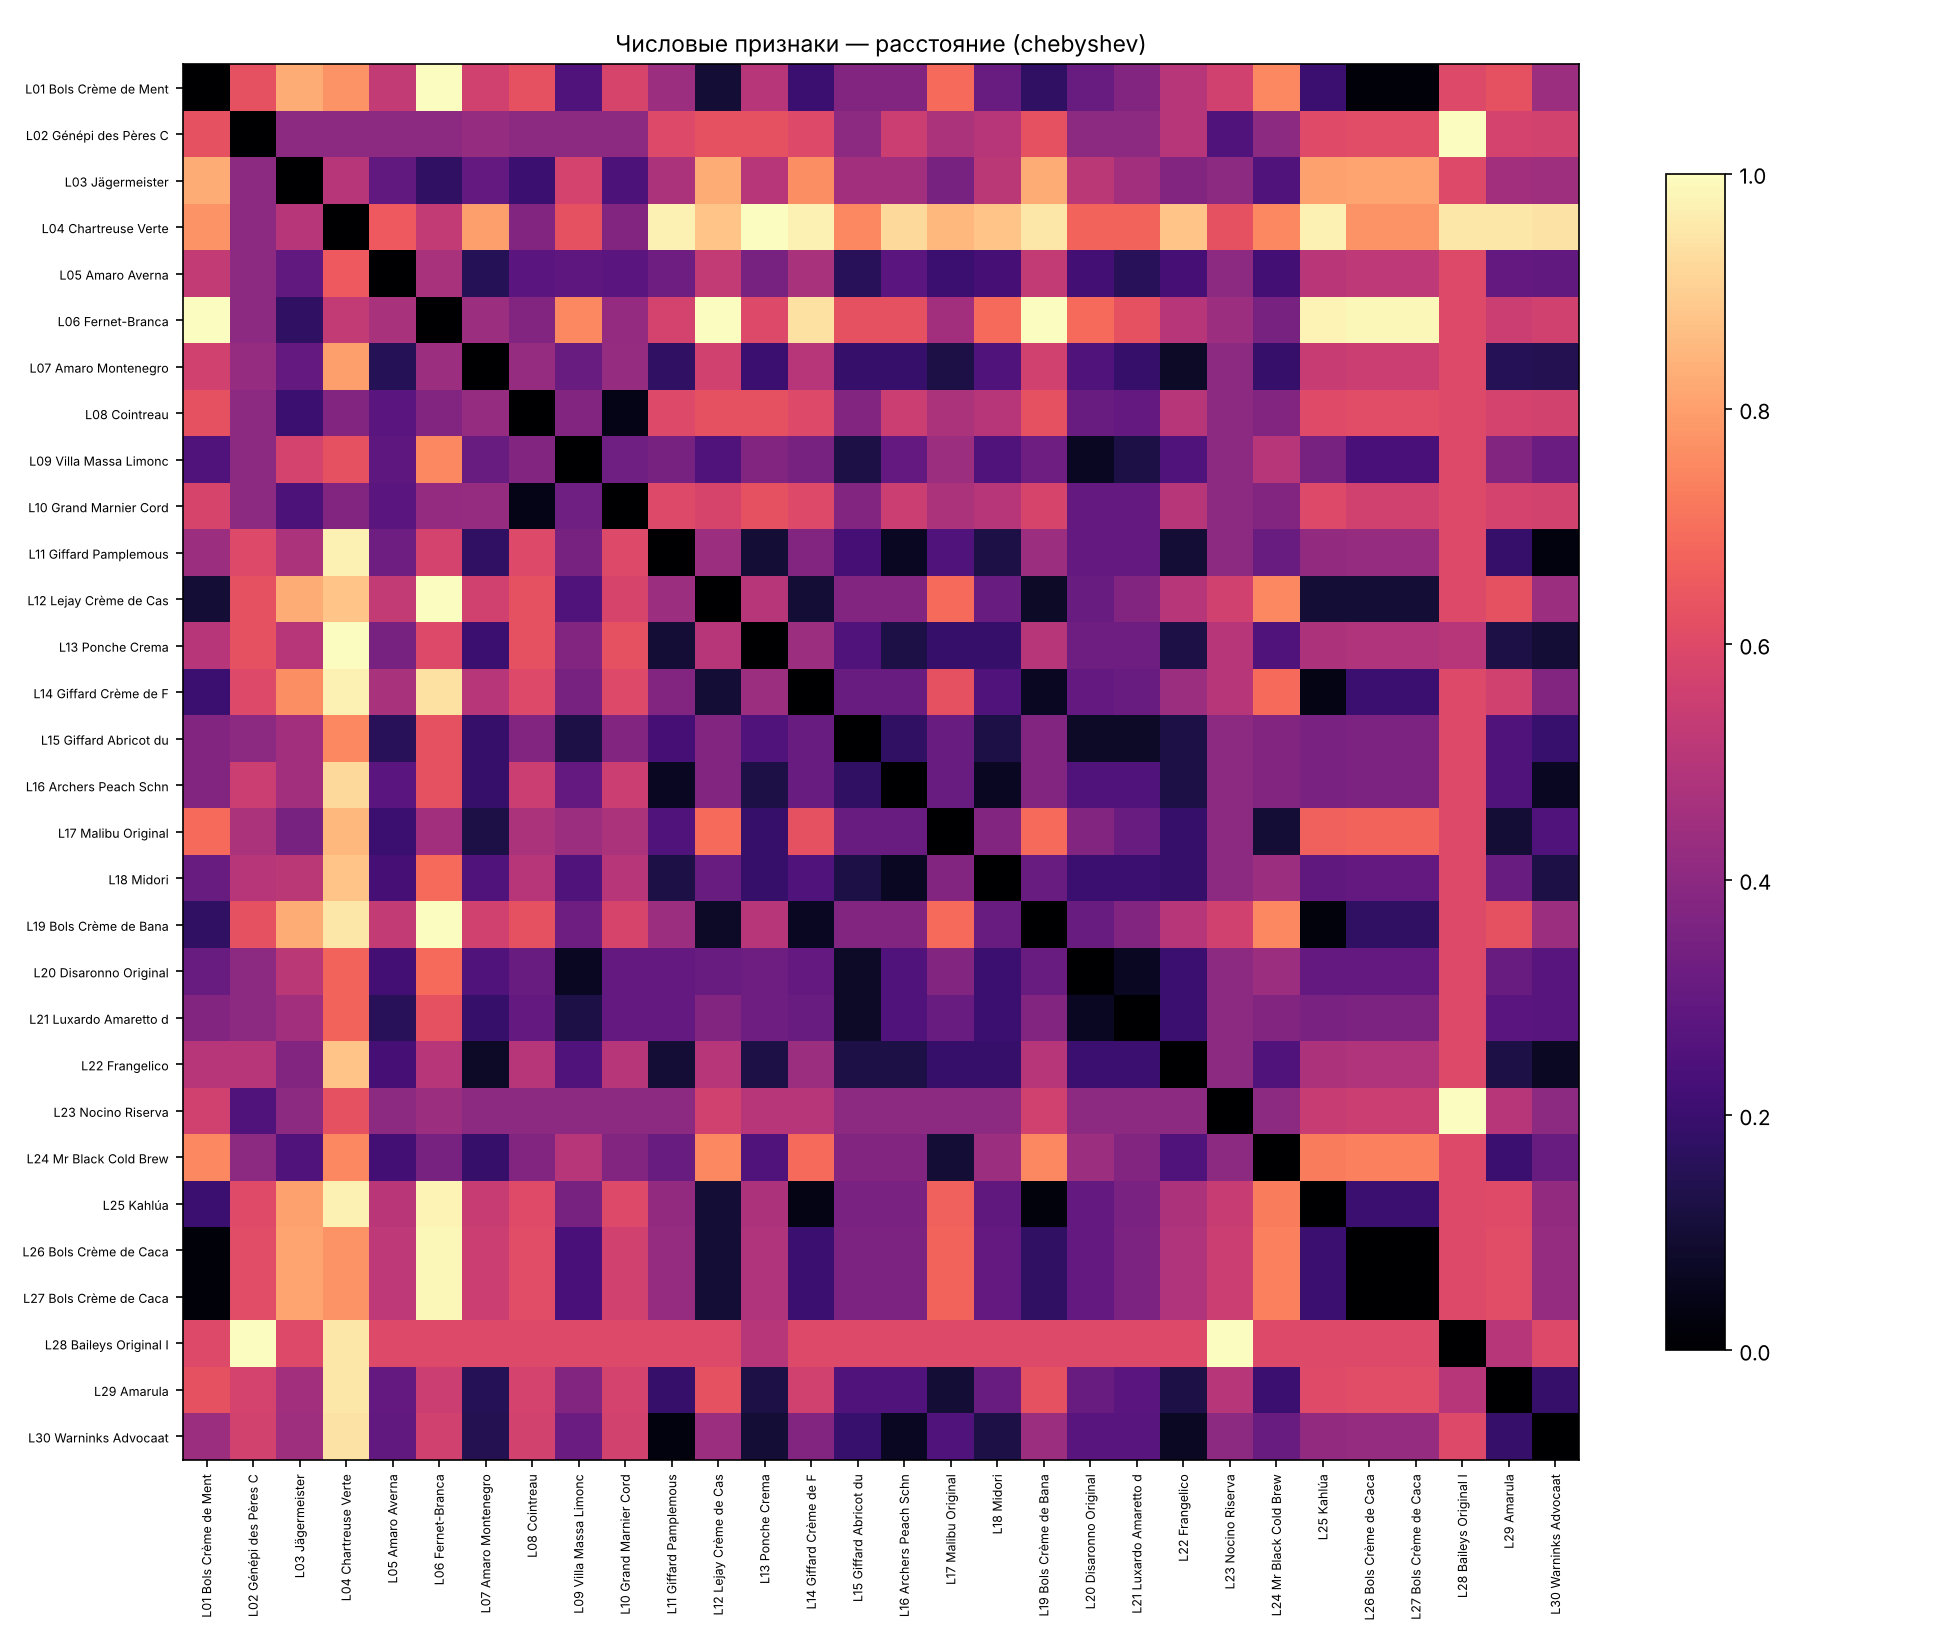
\includegraphics[width=0.32\textwidth]{lr2/num_chebyshev_dist.png}\hfill
	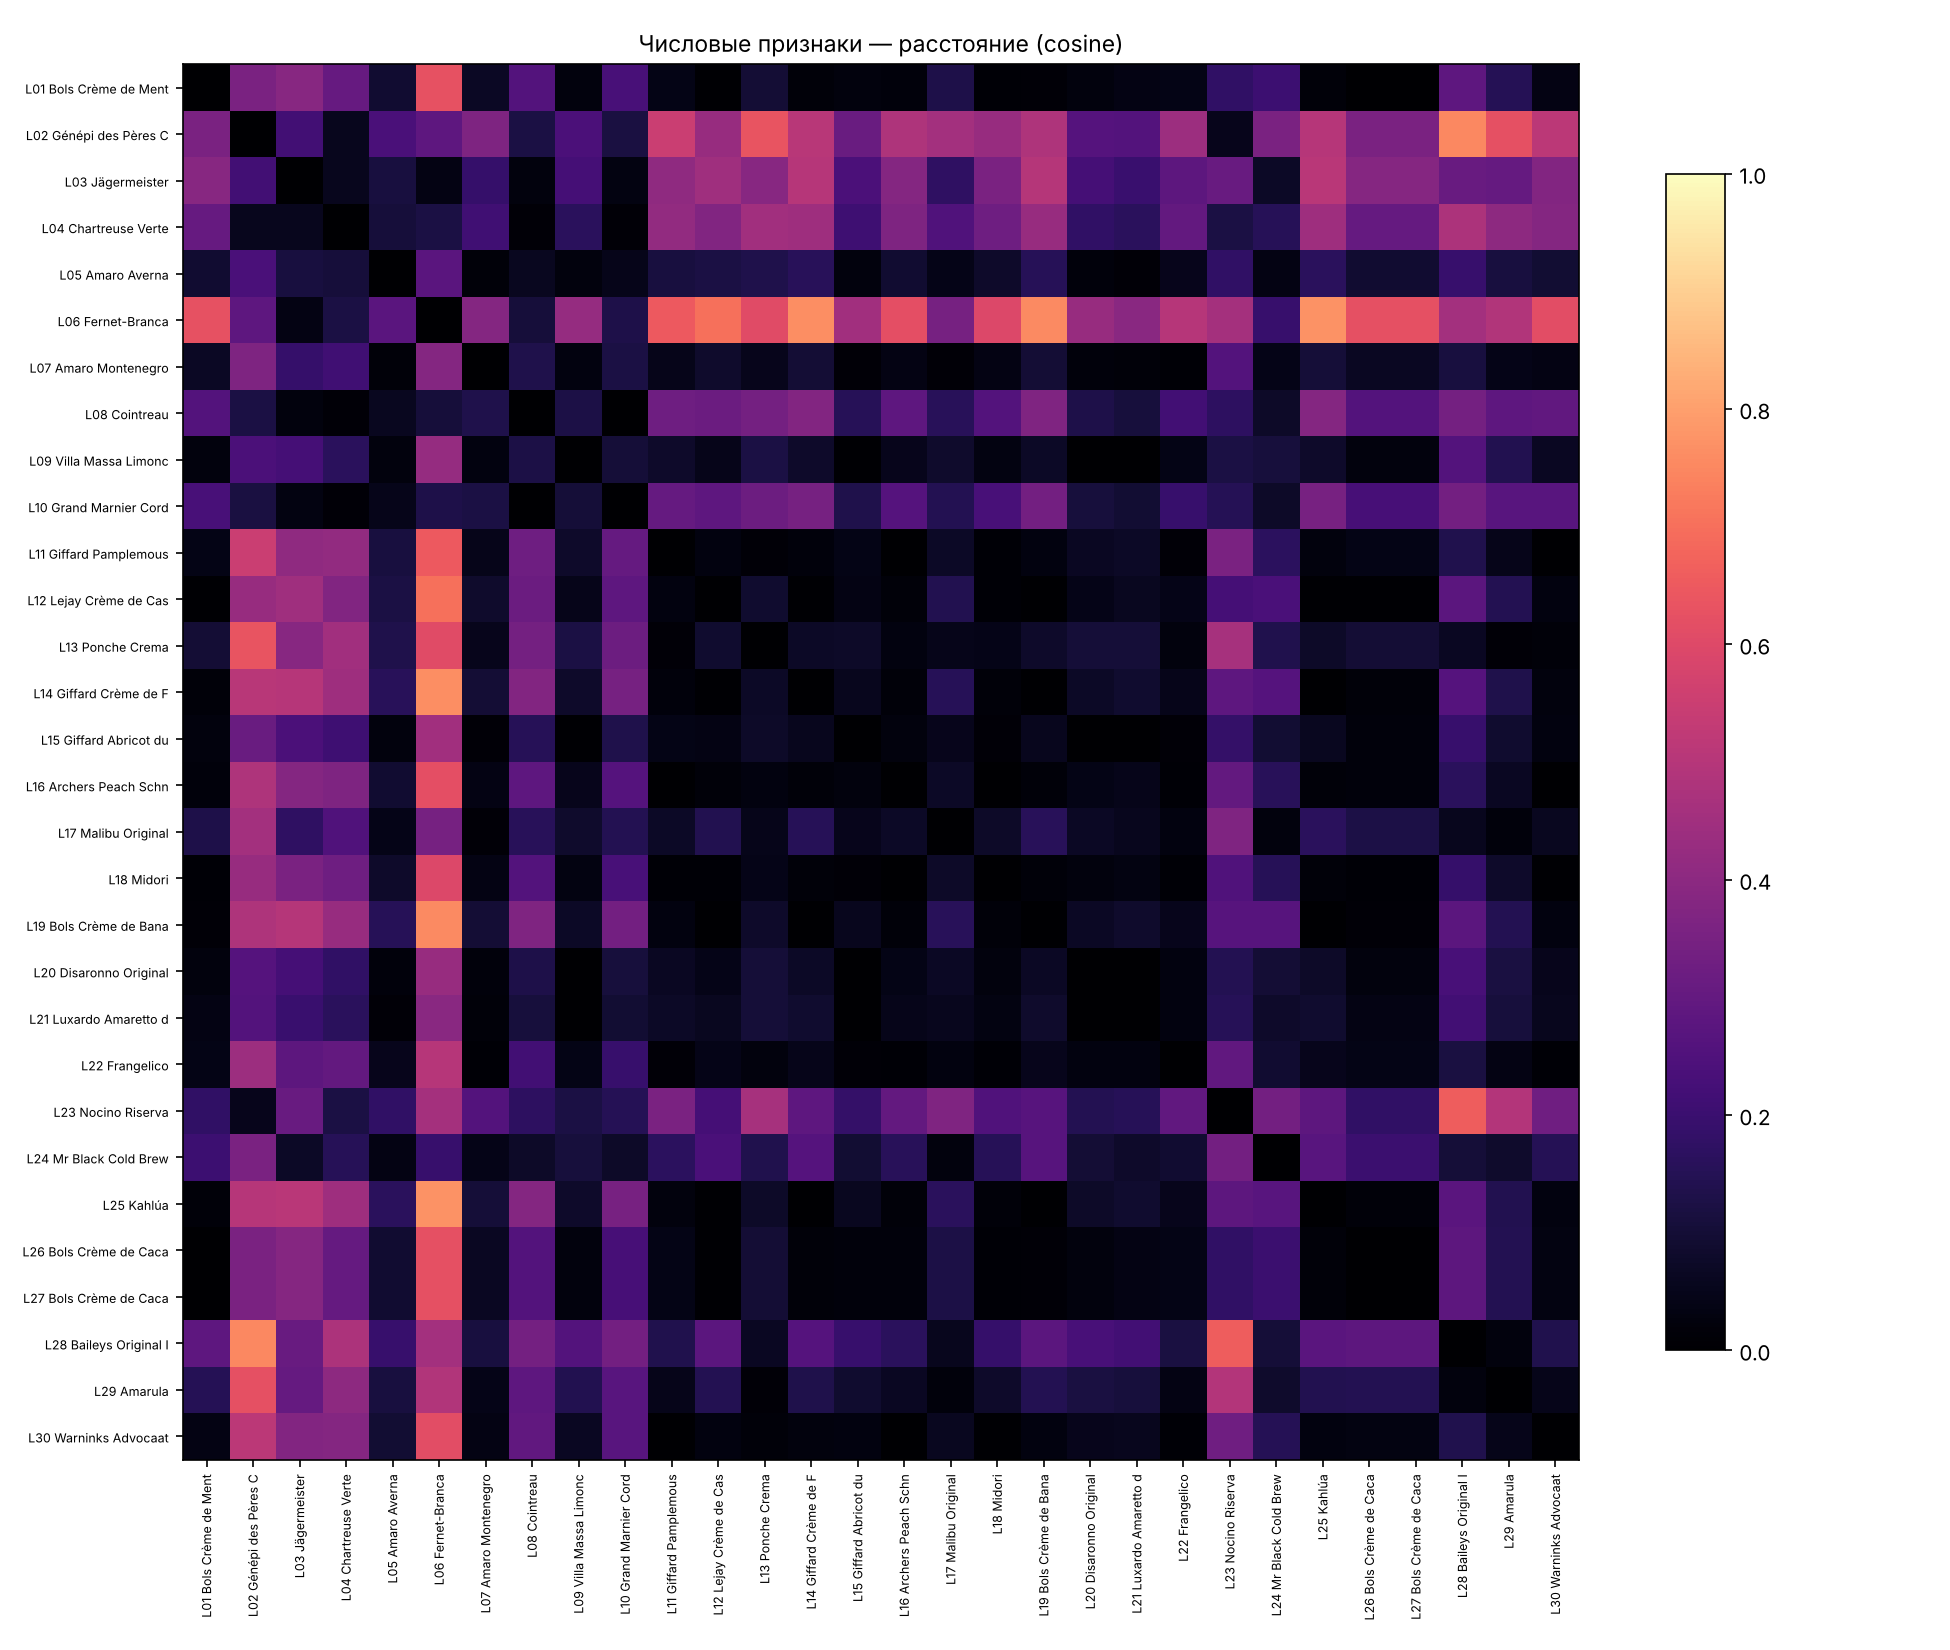
\includegraphics[width=0.32\textwidth]{lr2/num_cosine_dist.png}
	\caption{Тепловые карты числовых расстояний. Слева евклидово, в центре Чебышёва, справа косинусное}
	\label{fig:lr2_numeric}
\end{figure}

На рисунке~\ref{fig:lr2_numeric} видно, что карта Чебышёва ступенчатая. Косинусная карта почти однородно тёмная, потому что почти все пары для неё близки. Итоговая частная мера имеет вид $\mathrm{sim}_{num} = 1 - \sqrt{\tfrac13\sum_k (x'_k - y'_k)^2}$.

\section{Бинарные признаки}

Для вектора $(\code{bitter}, \code{wood\_contact})$ рассмотрены ассоциативные меры на таблице сопряжённости~\cite{volkova2014}. Здесь $a$ --- число совпадающих единиц, $b$ и $c$ --- рассогласования, $d$ --- число совпадающих нулей и $n = a+b+c+d = 2$. Меры записываются как Жаккар $a/(a+b+c)$, Дайс $2a/(2a+b+c)$, Сокал--Миченер (SMC) $(a+d)/n$ и Роджерс--Танимото $(a+d)/(a+d+2(b+c))$.

\begin{table}[H]
	\centering
	\caption{Бинарные меры близости на тестовых парах}
	\label{tab:lr2_binary}
	\footnotesize
	\begin{tabular}{|l|c|c|c|c|c|}
		\hline
		Пара & Векторы & Жаккар & Дайс & SMC & Роджерс--Танимото \\ \hline
		L26--L27 & (0,0)$\cdot$(0,0) & 0/0 $\Rightarrow$ 1* & 0/0 $\Rightarrow$ 1* & 1,000 & 1,000 \\ \hline
		L28--L30 & (0,1)$\cdot$(0,0) & 0,000 & 0,000 & 0,500 & 0,333 \\ \hline
		L05--L01 & (1,1)$\cdot$(0,0) & 0,000 & 0,000 & 0,000 & 0,000 \\ \hline
	\end{tabular}
\end{table}

У 19 из 30 ликёров вектор равен $(0,0)$. Это десертный стиль без горечи и выдержки, и для таких данных совпадение нулей содержательно. \textbf{Жаккар и Дайс отвергнуты}, потому что они игнорируют $d$ и на паре $(0,0)\cdot(0,0)$ дают неопределённость $0/0$, что видно из таблицы~\ref{tab:lr2_binary}. Baileys и Advocaat получили бы у них близость 0, хотя различаются одним признаком. \textbf{Роджерс--Танимото отвергнута.} При двух признаках двойной штраф сжимает шкалу, и одно различие даёт близость 1/3. \textbf{Выбран SMC}, доля совпавших признаков. Мера линейна и интерпретируема, у неё нет неопределённостей и выполнены все требования к близости. Если позже появятся длинные разреженные бинарные векторы вроде тегов-ингредиентов, выбор стоит пересмотреть в пользу Жаккара.

\section{Мера по таксономии вкуса}
\label{sec:lr2_taxonomy}

Признак \code{taste} --- лист дерева из ЛР1. $\delta$-функция <<совпал лист или нет>> потеряла бы структуру. Пары <<амаро--кройтер>> и <<амаро--банан>> обе получили бы 0. Поэтому нужна графовая мера на дереве. Рассмотрены три класса таких мер.
\begin{itemize}[leftmargin=1.6\parindent, label*=---]
	\item \textbf{Рёберные меры.} Это кратчайший путь $d = \mathrm{depth}(x)+\mathrm{depth}(y)-2\,\mathrm{depth}(\mathrm{LCA})$~\cite{rada1989}, мера Ликока--Чодороу на логарифме нормированного пути и мера У--Палмера $\mathrm{sim} = 2\,\mathrm{depth}(\mathrm{LCA})/(\mathrm{depth}(x)+\mathrm{depth}(y))$~\cite{wu-palmer}.
	\item \textbf{Узловые меры} по информативности узла $IC(c) = -\log p(c)$. Это меры Резника~\cite{resnik1995}, Лина~\cite{lin1998} и Цзяна--Конрата. Им нужны частоты понятий в корпусе. Оценивать частоты по 30 объектам ненадёжно, поэтому узловые меры отвергнуты.
	\item \textbf{Гибридные меры} Ли и др. Это нелинейная комбинация пути и глубины с двумя подгоночными параметрами. Для трёхуровневого дерева она избыточна.
\end{itemize}

\textbf{Выбрана мера У--Палмера.} В отличие от числа рёбер она учитывает глубину общего предка. Родство на уровне L2 конкретнее родства на уровне L1. Мера самонормирована в $[0,1]$ и даёт $\mathrm{sim}(x,x)=1$. Ей не нужны корпусные частоты, и она не меняет вид при добавлении уровня L4. Все листья лежат на глубине 3, поэтому мера принимает четыре значения из таблицы~\ref{tab:lr2_tax}. Она эквивалентна взвешенному общему пути с равными весами рёбер, а неравные веса уровней задаются параметрически.

\begin{table}[H]
	\centering
	\caption{Значения меры У--Палмера}
	\label{tab:lr2_tax}
	\footnotesize
	\begin{tabular}{|L{4.5cm}|c|c|L{6.3cm}|}
		\hline
		Общий предок & depth(LCA) & sim & Пример \\ \hline
		тот же лист L3 & 3 & 1,000 & L05--L07, оба <<Амаро>> \\ \hline
		общий L2, разные L3 & 2 & 0,667 & L26--L27, тёмный и белый шоколад \\ \hline
		общий L1, разные L2 & 1 & 0,333 & L01--L03, однотравный и сбор трав \\ \hline
		только корень & 0 & 0,000 & L08--L26, фруктовые и обжаренные \\ \hline
	\end{tabular}
\end{table}

\section{Порядковый и номинальные признаки}

Для лингвистической переменной \code{sugar\_class} из четырёх термов используется порядковая мера $\mathrm{sim} = 1 - |\mathrm{ord}(x)-\mathrm{ord}(y)|/3$. Соседние термы различаются на 1/3, а противоположные --- на 1. Номинальные признаки \code{country} и \code{producer} сравниваются $\delta$-функцией. Отношения порядка или иерархии между странами нет, а географическая близость не означает вкусовой. Италия и Франция производят ликёры всех ветвей дерева.

\section{Обобщающая мера}

Все частные меры имеют одну шкалу $[0,1]$. Поэтому их выпуклая комбинация
\begin{equation}
	\mathrm{sim}(x,y) = \sum_{k} \omega_k\,\mathrm{sim}_k(x,y), \qquad \sum_k \omega_k = 1,\ \omega_k \geq 0,
	\label{eq:lr2_total}
\end{equation}
сама является близостью в $[0,1]$ и даёт $\mathrm{sim}(x,x)=1$. Она учитывает все признаки, кроме служебных и текстовых. Экспертные веса и их обоснование приведены в таблице~\ref{tab:lr2_weights}.

\begin{table}[H]
	\centering
	\caption{Экспертные веса частных мер}
	\label{tab:lr2_weights}
	\footnotesize
	\begin{tabular}{|L{2.9cm}|L{2.9cm}|c|L{6.7cm}|}
		\hline
		Частная мера & Признаки & $\omega$ & Обоснование \\ \hline
		У--Палмер & taste & 0,35 & вкус --- главный смысл рекомендации ликёра \\ \hline
		евклидова & abv, sugar, volume & 0,30 & крепость и сладость --- второй по важности фактор выбора \\ \hline
		SMC & bitter, wood & 0,15 & заметные, но грубые модификаторы вкуса \\ \hline
		порядковая & sugar\_class & 0,10 & производный признак, вес занижен, чтобы не считать сладость дважды \\ \hline
		$\delta$-функция & country & 0,05 & слабый маркер стиля \\ \hline
		$\delta$-функция & producer & 0,05 & маркер линейки вроде серии Bols cr\`eme \\ \hline
	\end{tabular}
\end{table}

Экспертные веса нужно проверить на устойчивость. Для этого рассчитаны пять схем весов, не использующих экспертное знание. Это равные веса $1/6$, веса пропорционально числу признаков в блоке, веса по энтропии Шеннона распределения значений меры~\cite{shannon1948}, веса по среднеквадратическому отклонению и метод CRITIC по произведению контрастности и конфликта~\cite{critic1995}. Полученные веса показаны на рисунке~\ref{fig:lr2_weights}, а сравнение итоговых матриц --- в таблице~\ref{tab:lr2_schemes} и на рисунке~\ref{fig:lr2_schemes}.

\begin{figure}[H]
	\centering
	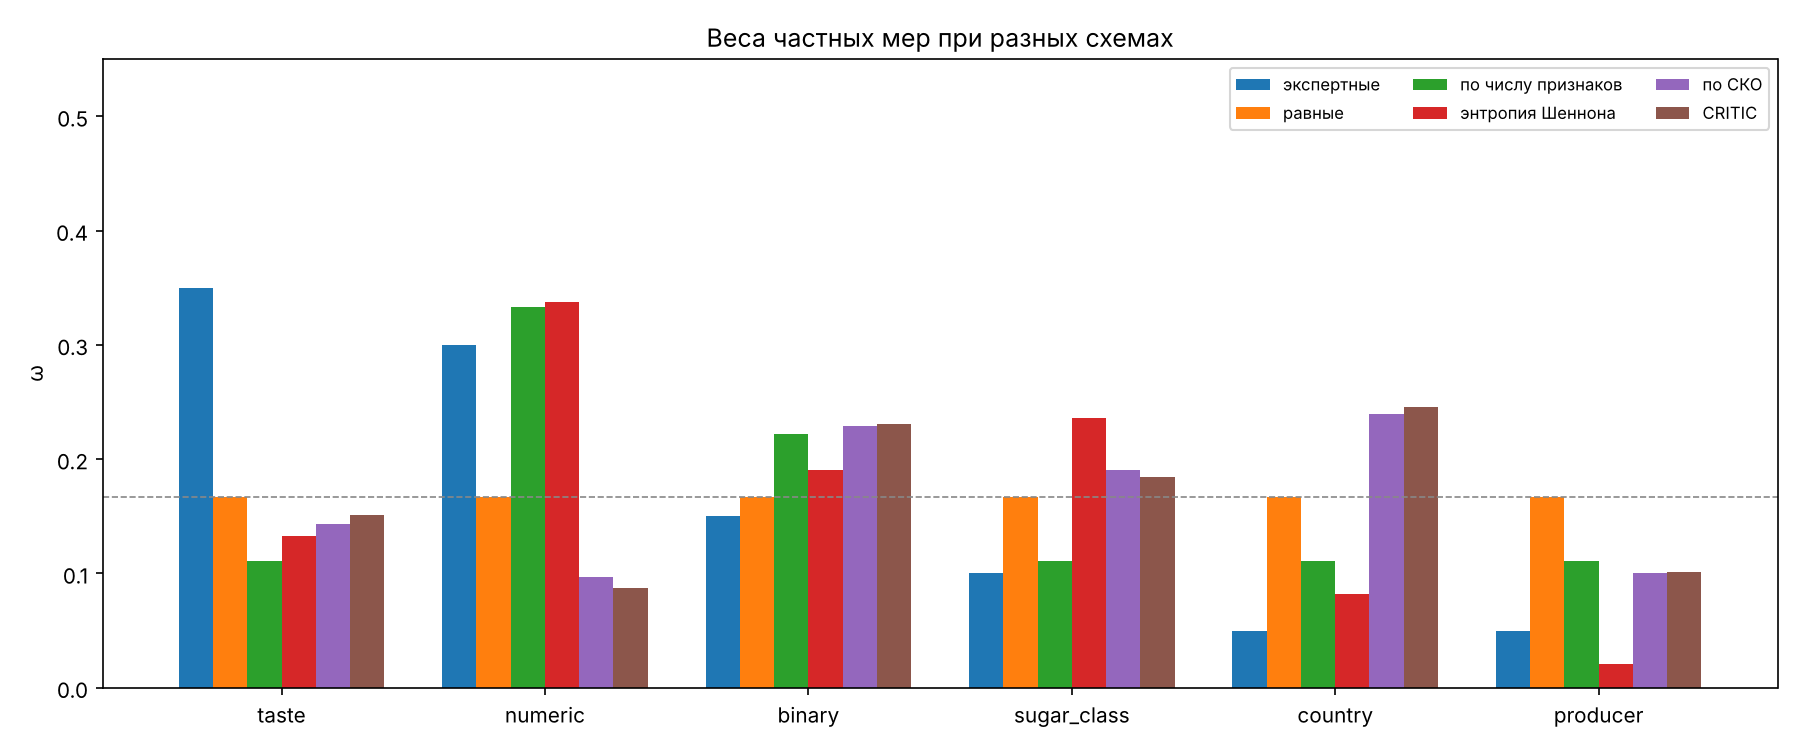
\includegraphics[width=0.9\textwidth]{lr2/agg_weights_bar.png}
	\caption{Веса частных мер при разных схемах}
	\label{fig:lr2_weights}
\end{figure}

\begin{table}[H]
	\centering
	\caption{Отличие итоговых мер от экспертной. Всего 435 пар}
	\label{tab:lr2_schemes}
	\footnotesize
	\begin{tabular}{|l|c|c|c|L{3.4cm}|}
		\hline
		Схема весов & Спирмен $\rho$ & средн. $|\Delta|$ & макс. $|\Delta|$ & Объектов с другим ближайшим соседом \\ \hline
		по числу признаков & 0,951 & 0,075 & 0,239 & 6 из 30 \\ \hline
		энтропия Шеннона & 0,937 & 0,125 & 0,244 & 9 из 30 \\ \hline
		равные & 0,925 & 0,061 & 0,232 & 7 из 30 \\ \hline
		по СКО & 0,883 & 0,067 & 0,261 & 8 из 30 \\ \hline
		CRITIC & 0,883 & 0,073 & 0,264 & 8 из 30 \\ \hline
	\end{tabular}
\end{table}

\begin{figure}[H]
	\centering
	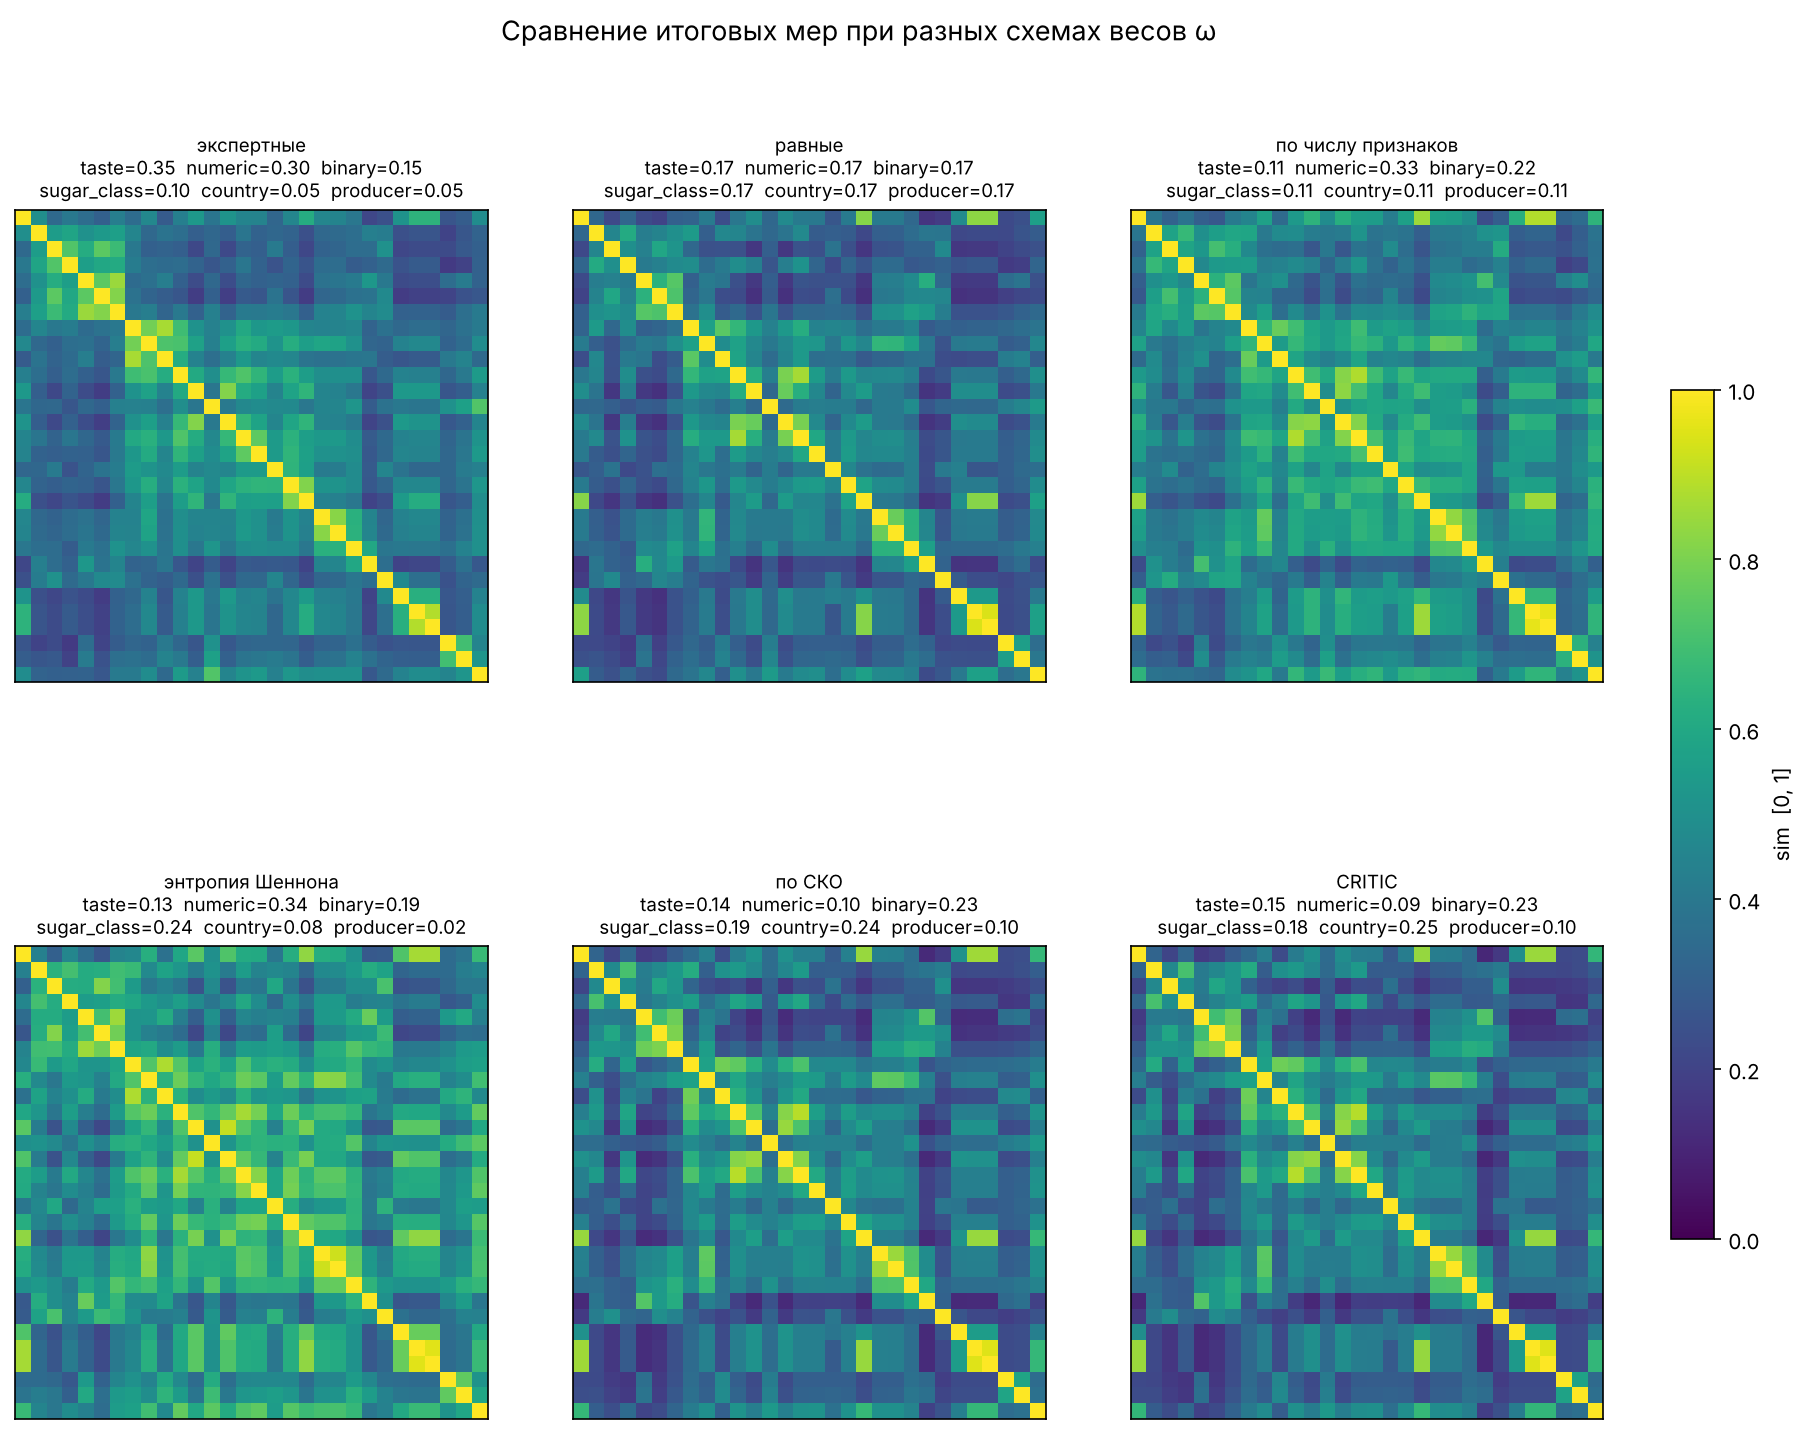
\includegraphics[width=0.8\textwidth]{lr2/agg_schemes_compare.png}
	\caption{Итоговые матрицы близости при шести схемах весов на общей шкале}
	\label{fig:lr2_schemes}
\end{figure}

Канонические <<двойники>> не распадаются ни в одной схеме. Это два какао-ликёра, два амаро, Cointreau и Grand Marnier, Baileys и Amarula. Они близки сразу по нескольким частным мерам. Меняется только второй ряд соседей. СКО и CRITIC дают стране вес около 0,24 вместо 0,05, потому что $\delta$-функция статистически контрастна. В ней много нулей и редкие единицы. В результате Limoncello отходит от Cointreau к Disaronno по общей стране Италии, хотя с Cointreau у него общий лист <<цедровые>>. Энтропия, наоборот, почти обнуляет производителя и завышает класс сладости. Последний коррелирует с числовым блоком, $r = 0{,}54$. Вывод прост. Объективные схемы измеряют контрастность шкалы, а не смысл рекомендации. Экспертные веса оставлены основными, а альтернативные схемы использованы как проверка устойчивости.

\begin{figure}[H]
	\centering
	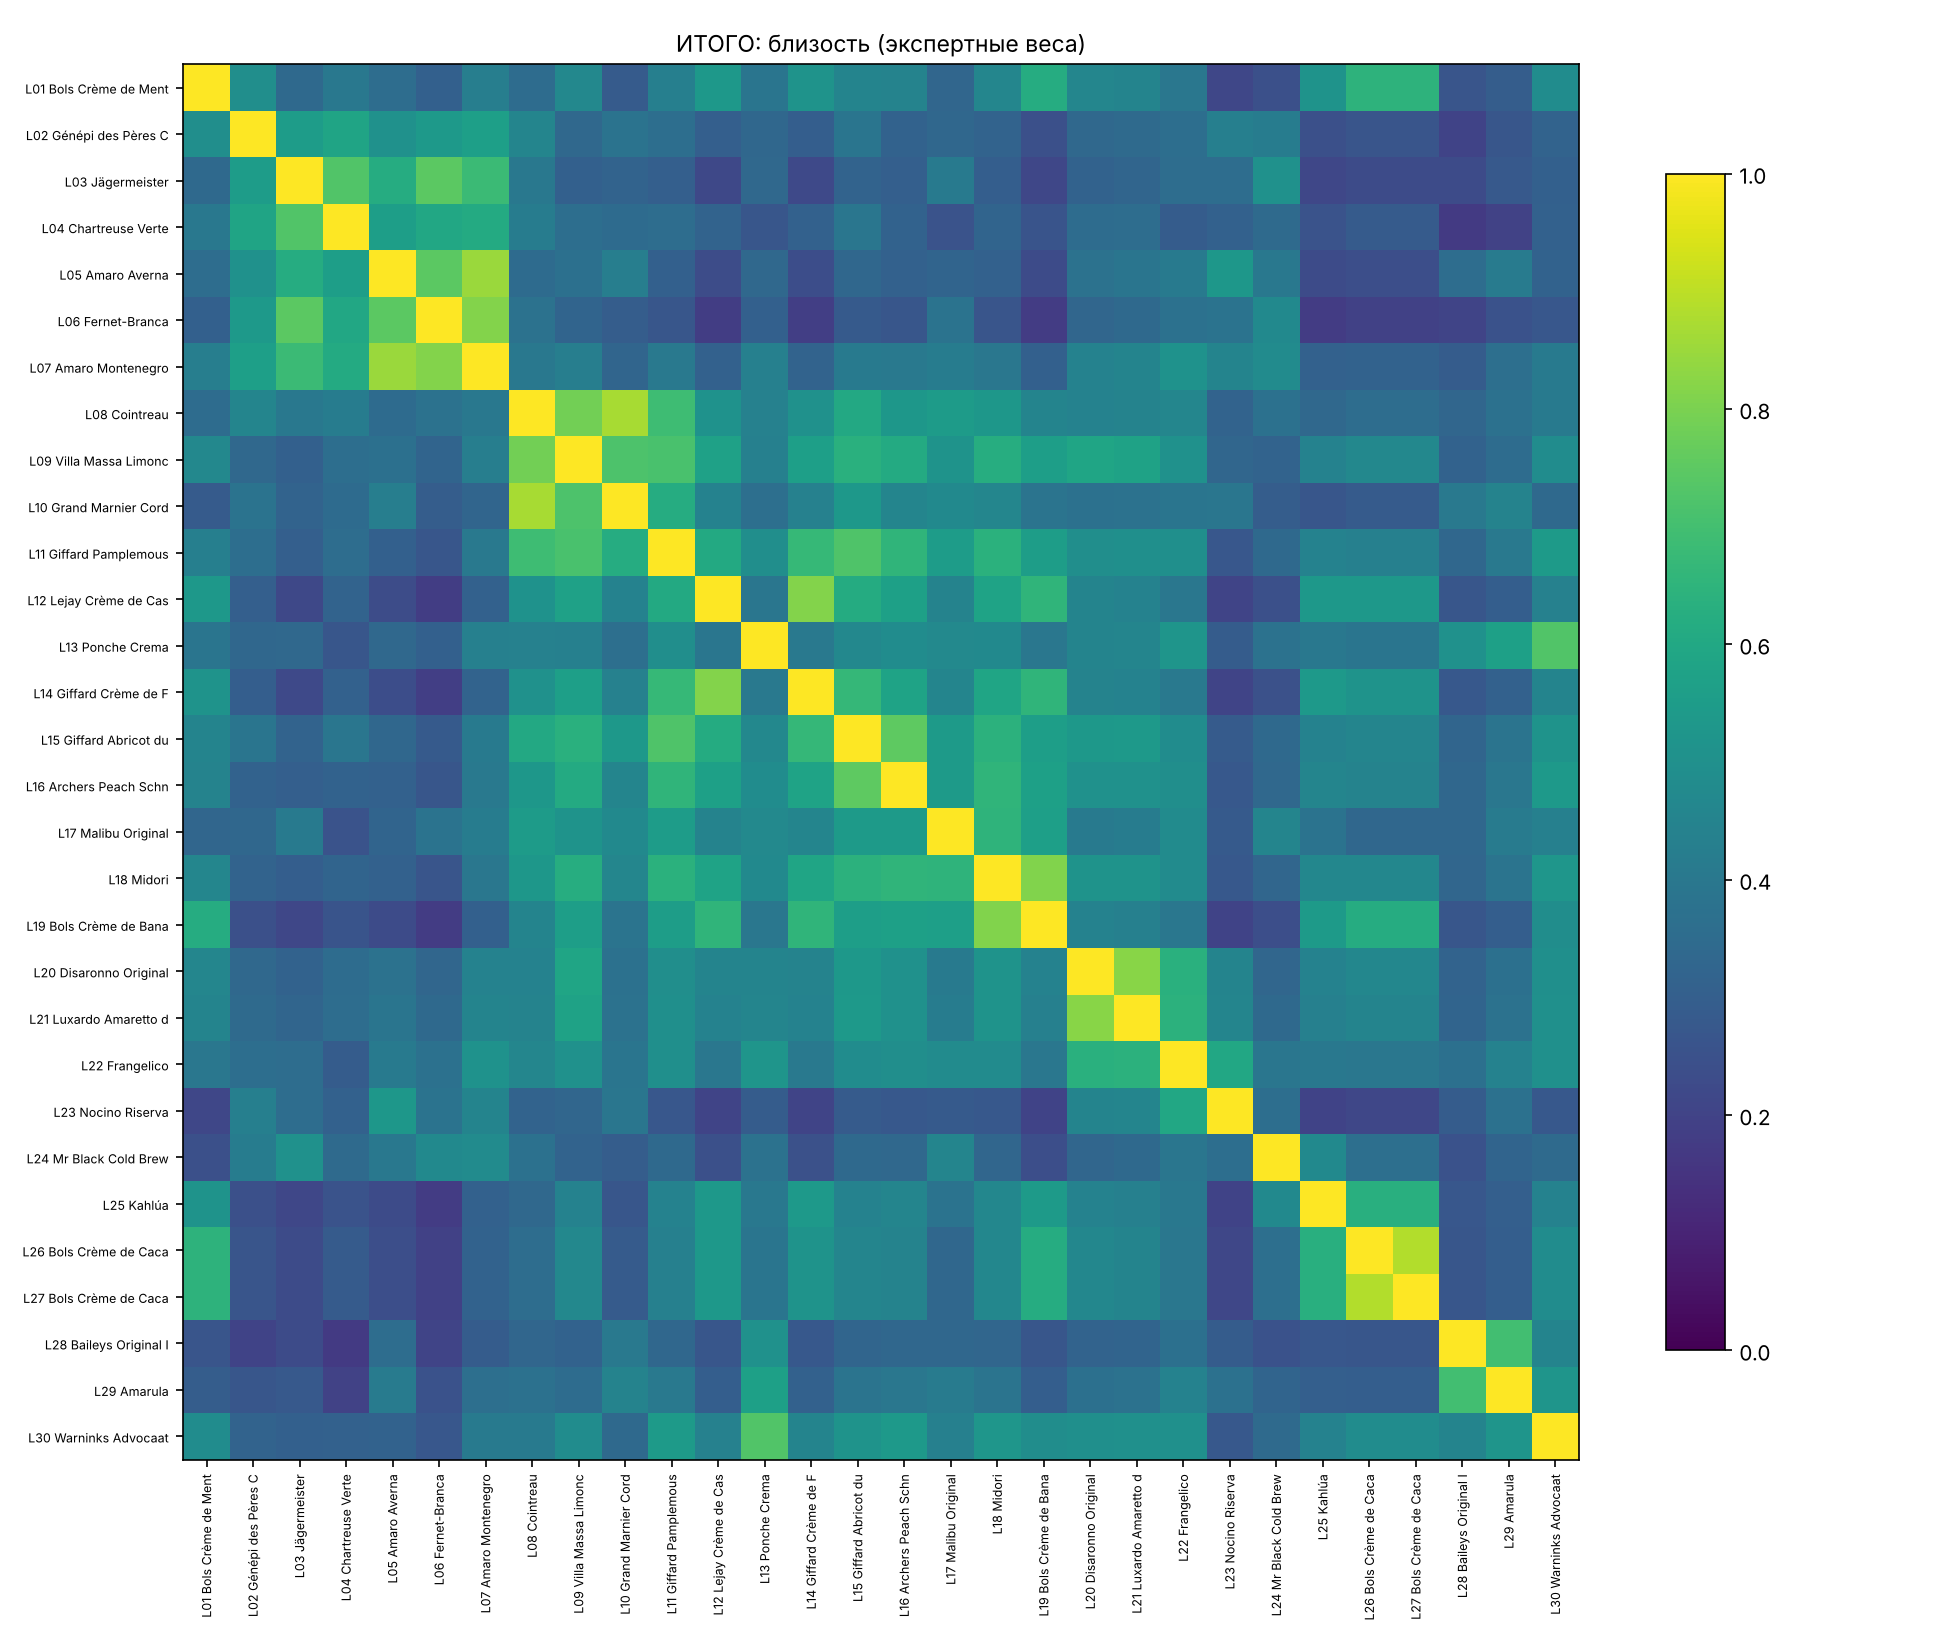
\includegraphics[width=0.62\textwidth]{lr2/agg_total_sim.png}
	\caption{Итоговая матрица близости с экспертными весами}
	\label{fig:lr2_total}
\end{figure}

На итоговой карте на рисунке~\ref{fig:lr2_total} видны блоки ветвей таксономии. Это травяные L01--L07, цедровые L08--L11, какао L26--L27 и сливочные L28--L29. Ближайшие соседи по итоговой мере экспертно верны и показаны в таблице~\ref{tab:lr2_nn}. Максимум вне диагонали равен 0,883, поэтому разные объекты не слипаются в 1.

\begin{table}[H]
	\centering
	\caption{Ближайшие соседи по итоговой мере}
	\label{tab:lr2_nn}
	\footnotesize
	\begin{tabular}{|L{4cm}|L{11cm}|}
		\hline
		Ликёр & Три ближайших соседа и близость \\ \hline
		L26 Cr\`eme de Cacao Brown & L27 Cacao White (0,883), L01 Cr\`eme de Menthe (0,647), L25 Kahl\'ua (0,632) \\ \hline
		L05 Amaro Averna & L07 Montenegro (0,848), L06 Fernet-Branca (0,750), L03 J\"agermeister (0,618) \\ \hline
		L08 Cointreau & L10 Grand Marnier (0,867), L09 Limoncello (0,789), L11 Pamplemousse (0,691) \\ \hline
		L28 Baileys & L29 Amarula (0,696), L13 Ponche Crema (0,504), L30 Advocaat (0,453) \\ \hline
		L24 Mr Black & L03 J\"agermeister (0,505), L07 Montenegro (0,483), L25 Kahl\'ua (0,476) \\ \hline
	\end{tabular}
\end{table}

\section*{Выводы}
\addcontentsline{toc}{section}{Выводы}

Для каждого типа признаков выбрана частная мера по формальной методике. Она включает матрицы смежности, тепловые карты, эталонные пары, согласованность ранжирований и зернистость шкалы. Выбраны нормированная евклидова мера для числовых признаков, SMC для бинарных, мера У--Палмера для таксономии вкуса, порядковая мера для класса сладости и $\delta$-функция для номинальных признаков. Обобщающая мера --- взвешенная сумма с экспертными весами. Её устойчивость подтверждена сравнением с пятью объективными схемами весов. Эта мера --- основа всех рекомендаций ЛР3 и функции полезности ЛР4.
